\section{First}\label{Sec:First}

We added another way to visiualize the volumes.
We thought that it would be nice to visualize the first voxel along each viewing ray.

Unfortunately this did not really work out, because for each volume there were different threshold for which we should choose that voxels as first voxel.
Because of this, we decided to add another slider in the settings panel so that the user can select the minimal value for the first voxel.
This way, the 'first' option becomes useful for all volumes.

As you can see in Figure~\ref{fig:first} we show the first voxel along the view ray that is at least 100.

\begin{figure}[H]
	\centering
		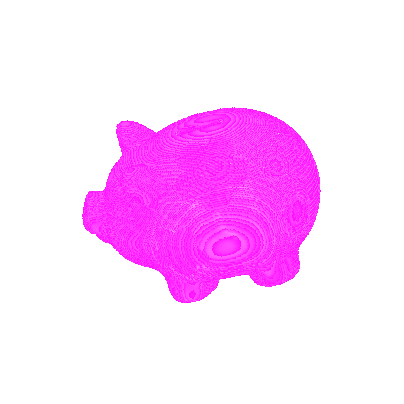
\includegraphics[width=0.6\textwidth]{pig_first}
		\caption{Shows the first values of \texttt{pig.fld} that are greater or equal to 100}
	\label{fig:first}
\end{figure}
